% Created 2011-10-17 Mon 12:27
\documentclass[12pt,a4paper]{article}
\usepackage[top=2cm,bottom=3cm,left=3cm,right=3cm]{geometry}
\usepackage{listings}
\usepackage{graphicx}
\graphicspath{{./figs/}{../figs/}{./}{../}} %note that the trailing / is required
\usepackage{indentfirst}
\usepackage[indentafter,pagestyles]{titlesec}
\usepackage{xltxtra}
\usepackage{xeCJK}
\usepackage{hyperref}
\usepackage[utf8]{inputenc}
\usepackage{fixltx2e}
\usepackage{longtable}
\usepackage{float}
\usepackage{wrapfig}
\usepackage{soul}
\usepackage{marvosym}
\usepackage{wasysym}
\usepackage{latexsym}
%\usepackage{amsmath,amsfonts,amssymb}
\tolerance=1000
\setlength{\parindent}{2.5em}
\setmainfont{DejaVu Serif}
\setsansfont{DejaVu Sans}
\setmonofont{DejaVu Sans Mono}
\setCJKmainfont[BoldFont={WenQuanYi Zen Hei}]{SimSun}
\setCJKfamilyfont{hei}{WenQuanYi Zen Hei}
\setCJKfamilyfont{song}{SimSun}
\XeTeXlinebreaklocale "zh"
\XeTeXlinebreakskip = 0pt plus 1pt
\renewcommand{\contentsname}{目录}
\renewcommand{\listfigurename}{插图目录}
\renewcommand{\listtablename}{表格目录}
\renewcommand{\abstractname}{摘要}
\renewcommand{\appendixname}{附录}
\renewcommand{\indexname}{索引}
\renewcommand{\figurename}{图}
\renewcommand{\tablename}{表}
\renewcommand{\refname}{参考文献} % article.cls 
\providecommand{\alert}[1]{\textbf{#1}}

\title{Linux简史}
\author{Ragib Hasan (翻译:王晓林)}
\date{作于:2002年7月; 译于:2006年1月}

\begin{document}

\maketitle

\setcounter{tocdepth}{2}
\tableofcontents
\vspace*{1cm}

\clearpage
\section{混沌初开}
\label{sec-1}

  那是在一九九一年,令人痛苦难耐的冷战渐渐走到了尽头,和平安详的空气开始升起在地平线。在计算科学领域,随着强大硬件的推出,计算机的极限能力已超出了我们的想象,一个辉煌的未来似乎已渐露端倪。
  
  但还是缺了点儿什么。在操作系统领域,存在着一片巨大的空白。

  一方面, \href{http://en.wikipedia.org/wiki/MS-DOS}{DOS} 还统治着庞大的个人电脑王国。\href{http://en.wikipedia.org/wiki/Bill_Gates}{比尔-盖茨} 花\$50,000从一个西雅图黑客手中买来DOS。之后,靠着聪明的市场策略,这个简陋的操作系统悄悄渗透到了世界的每一个角落。PC用户没有其它的选择。苹果机虽好,但它的天价没人能承受得起。它和大众需求保持着遥不可及的距离。

  计算领域的另一个阵营是 \href{http://en.wikipedia.org/wiki/UNIX}{UNIX} 世界。但UNIX更是贵不可攀。为了追求高额利润,UNIX销售商把价码抬得足以吓跑随便哪个PC用户。贝尔实验室曾慷慨地提供UNIX的源代码给大学。但现在,这些源代码被小心地看管起来,不再对外公开。更令全球PC用户心烦的是,软件市场的大玩家们没能为这一问题提供个有效的解决方案。

  \href{http://en.wikipedia.org/wiki/MINIX}{MINIX} 似乎是个选择。它是在荷兰当教授的美国人 \href{http://cs.vu.nl/~ast}{Andrew S.Tanenbaum} 从零开始编写出来的。MINIX的初衷是为了向学生讲授操作系统的内部工作原理。MINIX的设计是面向当时最为流行的Intel8086微处理器。作为一个操作系统,MINIX算不上一流。但它的好处是你能得到它的源代码。只要你有Tanenbaum写的《操作系统:设计与实现》这本书,你就能得到那12,000行用C和汇编写的源码。头一次,程序员或黑客可以有机会读一读操作系统的源码--这种被软件商严加看管的东西。Tanenbaum用详尽简洁的笔触探讨了编写操作系统的艺术。他是个一流的作者,迷住了一批当时计算机领域最聪明的大脑。全世界学计算机的学生都在钻研这本书,通过读它的源码来了解他们电脑里运行的MINIX操作系统。

  Linus Torvalds就是这些学生中的一个。
\section{呱呱坠地}
\label{sec-2}

  在1991年, \href{http://www.cs.helsinki.fi/~torvalds/}{Linus Benedict Torvalds} 还是个芬兰学生,在\href{http://www.hut.fi}{赫尔辛基大学} 念计算机专业二年级。同时他也是个自学成才的黑客。这个长着沙滩黄头发,说话软绵绵的二十一岁芬兰帅哥喜欢折腾他的电脑,把它不断推向能力的极限。但他缺少一个合适的操作系统来满足他如此专业的需求。MINIX不错,可它只适合学生,是个教学工具,而不是一个强大的实战系统。

  当时,全世界的程序虫们都很看好 \href{http://www.stallman.org/}{Richard Stallman} 的 \href{http://www.gnu.org/}{GNU} 项目---一个致力于推出自由、高质量软件的运动。在计算科学的王国里,Stallman是个倍受尊崇的神话式英雄。他令人景仰的职业生涯是从大名鼎鼎的MIT人工智能实验室开始的。

  七十年代中后期,他在那里开发出了著名的\href{http://en.wikipedia.org/wiki/Emacs}{Emacs} 编辑器。八十年代早期,商业软件公司从人工智能实验室吸引走了绝大多数优秀的程序员,并和他们签署了严格的保密合同。Stallman为此大大不爽。他认为软件和其它产品不同,在复制和修改方面它不该受到任何限制。只有这样,才能开发出更好更强的软件。1983年,他在著名的《GNU宣言》中,向世人宣告了GNU项目的启动,开始了贯彻其哲学的自由软件运动(顺带一句,GNU一词是 ‘GNU's Not Unix’ 的递归缩写)。 为了最终实现开发出一个自由操作系统的梦想,他得先制造些工具。于是,在1984年初,Stallman开始创作一个令商业企业程序员叹服的作品 --- \href{http://en.wikipedia.org/wiki/GNU_Compiler_Collection}{GNU C编译器} (gcc)。他出神入化的技术天才,令所有商业软件程序员自愧不如。gcc被公认为世界上最高效最强健的编译器之一。

  \begin{figure}[h!]
  \centering
  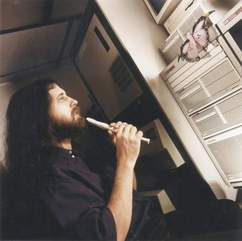
\includegraphics[width=0.38\textwidth]{./figs/stallman.png}
  \caption{Richard Stallman,GNU项目的创始人}
  \end{figure}

  到1991年,GNU项目已经开发出了众多的工具软件。大家期待已久的 GNU C 编译器也问世了。但自由操作系统还没有出现。MINIX也是受版权约束的(后来,在2000年4月,Tanenbaum在BSD许可证下发布了自由的MINIX)。GNU操作系统内核 --- HURD --- 还在开发之中,几年之内还不可能面世。

  拖了这么久,终于该说说Linus了。

  1991年8月25号,Linus在MINIX新闻组发出了历史性的一贴\ldots{}

\begin{verse}
From: torvalds@klaava.Helsinki.FI (Linus Benedict Torvalds)\\
Newsgroups: comp.os.minix\\
Subject: What would you like to see most in minix?\\
Summary: small poll for my new operating system\\
Message-ID: <1991Aug25.205708.9541@klaava.Helsinki.FI>\\
Date: 25 Aug 91 20:57:08 GMT\\
Organization: University of Helsinki\\
\vspace*{1em}
Hello,各位使用minix的朋友,\\
\end{verse}

\begin{quote}
我正在写一个基于386(486)AT机器的(自由)操作系统(只是出于爱好,不会做得象gnu那么大、那么专业)。
我从四月份开始酝酿,现在已经做得差不多了。我现在想知道一些你们对minix的看法,它哪点好?哪点不好?
因为我这个操作系统和minix多少有点儿类似(文件系统采用同样的物理布局(因现实原因),
其它方面也有类似的地方)。我已经把bash(1.08)和gcc(1.40)移植过来了,而且它们运转正常。
这意味着在下面几个月里,我将给它加上更多实际的功能。所以我想知道大家都希望它有哪些功能。
欢迎多提建议,但我不敢保证能实现你的建议 :-)

Linus (torvalds@kruuna.helsinki.fi)

附:没错,它不包含任何minix的代码,而且它有一个多线程文件系统。
它现在不能在其它硬件上转(因为用了386任务切换机制,等等),而且除了AT硬盘,
它基本上不支持任何其它硬件。这就是全部了 :-(。
\end{quote}

  从这个帖子不难看出,Linus自己并没预料到他的小创造将会改变整个计算科学领域。1991年9月中旬, Linux 0.01 版问世了,并且被放到了网上。它立即引起了人们的注意。源代码被下载、测试、修改,最终被反馈给Linus。10月5号,0.02版出来了,同时伴随着Linus著名的声明:
\begin{verse}
From: torvalds@klaava.Helsinki.FI (Linus Benedict Torvalds)\\
Newsgroups: comp.os.minix\\
Subject: Free minix-like kernel sources for 386-AT\\
Message-ID: <1991Oct5.054106.4647@klaava.Helsinki.FI>\\
Date: 5 Oct 91 05:41:06 GMT\\
Organization: University of Helsinki\\
\end{verse}

\begin{quote}
你在怀念minix-1.1时代的美好时光吗?那时你自己写着驱动,充满了作男人的感觉。
现在没什么好项目可做了,是吗?你在拚命啃一个操作系统,修改它以满足你的需求,是吗?
现在minix已经没什么需要你去改进的了,你为此怅然若失,是吗?
没机会再熬通宵去改进一个小程序了,是吗?如果是这样的话,那这个帖子就是给你的 :-)

一个月(?)前我曾经提到过,我正在一个AT-386机器上开发一个自由版本的、类似minix的操作系统。
现在它终于出来了(尽管未必能满足你的期待)。我乐意把源代码公开出来,让它传播得更广。
它现在仅仅是0.02版(外加一个(很小的)补丁)。但是我已经成功地在它上面跑了
bash/gcc/gnu-make/gnu-sed/compress等程序。我这个小宝贝儿的源程序在
nic.funet.fi(128.214.6.100)下面的/pub/OS/Linux目录中可以找到。
该目录中还有些README文件,还有几个在linux下能工作的可执行文件(bash,update和gcc),
你还要求些什么呢:-)。完整的内核源代码都公布在这儿了,因为里面没用到minix的源程序。
而函数库的源程序只是部分开源,所以目前还不能提供出来。拿到源代码后,直接编译就行了。
编译完就能转了。哈哈。可执行程序(bash和gcc)的源代码可以在同一网站的/pub/gnu目录里找到。
\end{quote}

几周以后, Linux 0.03 版发布了。12月份,0.10版发布了。这时的Linux还显得很简陋。它只能支持AT硬盘,而且不用登录(启动就进bash)。0.11版有了不少改进,可以支持多国语言键盘、软驱、VGA、EGA、Hercules等等。Linux的版本号从0.12直接上升到了0.95、0.96\ldots{}不久,Linux的源代码就通过在芬兰和其它一些地方的FTP站点传遍了全世界。
\section{谁与争锋}
\label{sec-3}

  
  \begin{figure}[h!]
  \centering
  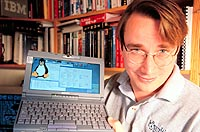
\includegraphics[width=0.38\textwidth]{./figs/laptop.png}
  \caption{Linus在展示一台Linux笔记本电脑}
  \end{figure}
  
  不久,Linus开始面对挑战。他面对的不是别人,正是Andrew Tanenbaum, 那个开发出MINIX的伟大教师。在给Linus的一个回贴中,Tanenbaum写到:
\begin{quote}
“我还是坚持我的观点,在1991年还设计这样一个整体架构的内核是个根本性的 错误。你该庆幸不是我的学生。这么个设计,在我这儿你得不了高分:-)”

(Andrew Tanenbaum to Linus Torvalds)
\end{quote}

  Linus后来承认说,这是关于开发Linux他所得到的最坏评价。Tanenbaum是当时的知名教授,他说的话自然很有份量。但这次面对Linux,他的话没能奏效,因为Linus不是个轻易服输的人。
  
  Tanenbaum还宣称:
\begin{verse}
“Linux过时了。”  \\
\end{verse}

  现在轮到新的Linux一代开始反击了。以强大的Linux社区为后盾,Linus给了Tanenbaum一个恰如其分的回复:
\begin{quote}
“你的工作是教授、研究员。这对于minix的大脑损伤是个绝妙的解释。”

(Linus Torvalds to Andrew Tanenbaum)
\end{quote}

  Linux的开发在继续。不久,加入开发的人数就超过了一百,然后是数千,然后是数十万。Linux不再只是个黑客的玩具,配合上GNU项目开发出的众多软件,Linux已经可以走向市场了。它最终在GNU公共许可证下发布,这保证任何人都可以自由获得它的源代码,可以自由复制、学习和修改它。学生和程序员们都没错过这个机会。

  不久,软件商们也来了。Linux是自由的操作系统。软件商们需要做的只是把各种各样的软件在Linux平台上编译,然后把它们组织成一种可以推向市场的形式。这和其它操作系统在运作模式上没什么区别,只是Linux是自由的。\href{http://redhat.com/}{Redhat}, Caldera, 和其它一些公司都获得了相当大的市场,获得了来自世界各地的用户。除了这些商业公司,非商业的编程专家们也志愿地组织了起来,推出了他们自己的品牌--享誉全球的\href{http://www.debian.org}{Debian}。 配上崭新的图形界面(比如\href{http://www.x.org/}{X Window System}, \href{http://www.kde.org/}{KDE}, \href{http://www.gnome.org/}{GNOME}), Linux的各个品牌都倍受欢迎。

  好戏连台,惊喜不断。除了PC机,Linux又被移植到了许多其它平台上(PowerPC、 Sun Sparc、ARM、Alpha\ldots{} Debian就支持十几种CPU)。它还被人安装到了3com的手掌计算机上。另外,利用集群技术,许多Linux单机可以被组织成一个整体,用于并行计算。1996年4月, Los Alamos 国家实验室的研究人员利用68台Linux单机搭建了一个并行计算系统,用它来模拟原子弹爆炸的冲击波。与其它超级计算机不同的是,用Linux搭建的集群计算机非常便宜。这种DIY出来的超级计算机只花费\$152,000,连人工(连接68台PC的线缆)都包括了。这价格只是同级别商业机的十分之一。它的峰值计算速度可达每秒190亿(19 billion, 19x10$^9$) 次。在世界超级计算机排行榜中它排在第315位。它也极其稳定可靠,投入运行三个月后,还不必去重启动。

  \begin{figure}[h!]
  \centering
  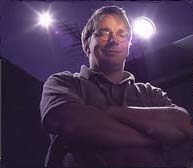
\includegraphics[width=0.38\textwidth]{./figs/linusnow2.png}
  \caption{今天锋芒毕露的Linus}
  \end{figure}

  今天,Linux最大的优势就是推动它前进的巨大开发热情。一旦有新硬件问世,Linux内核就能快速被改进以适应它。比如,Intel Xeon 微处理器才问世几个星期,Linux新内核就跟上来了。它还被用在了Alpha、MAC、PowerPC上。甚至在手掌机这一少人问津的领域都可以运行Linux。正如它在1991年诞生时那样,Linux正以同样的热情阔步走向新世纪。

  \begin{figure}[h!]
  \centering
  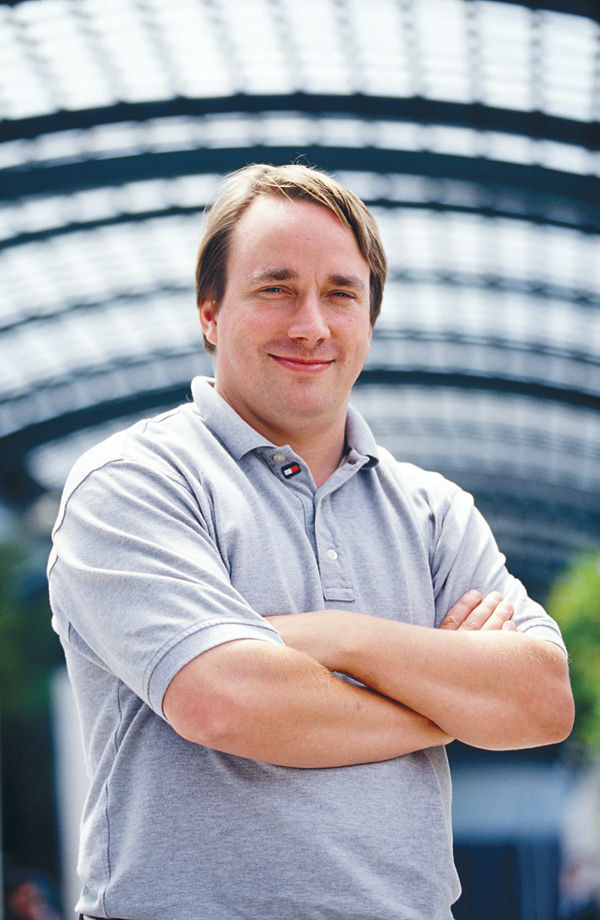
\includegraphics[width=0.38\textwidth]{./figs/Linus_Torvalds.png}
  \caption{Linus,2002}
  \end{figure}

  至于Linus本人,他保持着简单的生活。不象比尔盖茨,Linus不是亿万富翁。完成学业之后,他移居美国,在Transmeta公司找了个工作。Transmeta公司在指导完成了一个绝密项目的研发之后,推出了自己的Crusoe处理器。Linus是这个研发小组中活跃的一员。最近,他和Tove结了婚,生了个女儿,取名Patricia Miranda Torvalds。世界范围内的计算机社区都对Linus推崇备至,到目前为止,他是我们这个星球上最受欢迎的程序员。

  \begin{figure}[h!]
    \centering
    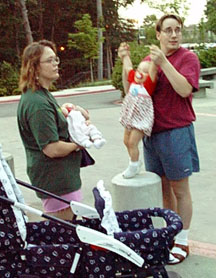
\includegraphics[width=0.38\textwidth]{./figs/family.png}
    \caption{全家福}
    \end{figure}  
\section{风雨十年}
\label{sec-4}

  Linux的开发已经走过了十个年头。它用十年的蓬勃发展否定了所有持怀疑态度的警告和预言。今天,Linux是有史以来发展速度最快的操作系统之一。从91、92年的几个技术狂热者发展到今天数以百万计的普通用户,这绝对是个不平凡的历程。大商业公司们“发现”了Linux,将数以百万计的美元倾入到开发中来,这一事实无情地驳斥了“开源运动反商业”的谬论。IBM曾经视开源社区为洪水猛兽。而现在,它已经将大量的资金转移到以Linux为平台的开源解决方案中来。

  但真正让人感到惊喜的是,Linux开发团队持续不断地壮大,并在世界范围内扩散开来。这些开发者以旺盛的精力和高涨的热情不断改进着Linux的功能和性能。Linux的开发工作并没有象“代码封闭论者”所妄言的那样“最终消失在一片混乱之中”。正相反,Linux的开发是有组织有秩序的,它采用的是一种精心设计并被细心维护的开发模式。在这一高效开发模式下,数以千计的开发者们把各种 各样的应用软件注入到Linux平台中来。

  商业企业不再对Linux心怀戒惧,因而大量的软件商开始提供Linux平台上的产品支持,软件质量有了更可靠的保障,在办公室里用Linux不必再有“风险自负”的担心了。说到可靠性,Linux在1999年CIH病毒肆虐和一年后的‘爱虫’病毒流行时,证明了自己的强健。这些相当简单的小病毒把世界搞得一团糟,而所有的Linux机器却丝毫不受影响。这充分显示了它出色的免疫力。当Redhat这样的Linux排头兵走向市场的时候,它们受到了热烈的欢迎。甚至在近几年dot-com网络泡沫破灭之后,它们还在持续蓬勃地发展壮大。这也大大增强了人们对Linux的信心,许多大大小小的商业公司开始采用Linux作服务器和工作站平台,把Linux作为办公室系统的可靠支撑。
\subsection{桌面应用}
\label{sec-4-1}

   那么,针对Linux人们报怨最多的是什么呢?在过去,也许就数它的字符界面了。很多对Linux感兴趣的人被传统的字符界面吓着了。“字符界面可以让你无所不能”,一些执着的黑客会向你这样辩解。但对于数百万的普通用户,这意味着要花费大量的时间和精力去学习它。现成的XWindow图形界面和窗口管理器并不能满足普通计算机用户的期待。这一直是MS Windows 追随者们的攻击把柄。但在过去的几年间,情况发生了改变。象KDE和GNOME这样非常专业的桌面环境呈现在了人们的面前。这些桌面环境的较新版本使人们对Linux的“用户友好性”有了更好的认识。尽管一些铁杆用户在报怨,图形化使黑客文化失去了其原有的纯正品味。但图形化大大改善了Linux在普通用户心目中的形象,促进了Linux的流行与推广。
\subsection{第三世界}
\label{sec-4-2}

   Linux在发展中国家得到了广泛的传播。这也许是它对世界影响最大的地方。在Linux出现之前,发展中国家在计算科学领域大大落后于西方。虽然硬件价格不断下滑,但在第三世界国家,计算机爱好者们饱有热情,却又囊中羞涩。软件的高昂价格一直是个巨大的经济负担。无奈中,他们只能求助于各种各样的盗版软件。这直接导致了盗版的泛滥,盗版金额高达数万亿美元。话又说回来,大多数商业软件的标价都大大超过了发展中国家人民的承受力。举例来说,一个典型的操作系统软件至少标价\$100。在一个年人均收入只有\$200-\$300的国家,这\$100是个巨额数字。

   Linux和其它开源软件的崛起彻底改变了这一切。在适当的裁减之后,Linux可以在硬件配置极低的计算机上运行。这使得Linux成为穷人的理想选择。在发达国家已经成为历史的老旧机器,比如486/Pentium1计算机,在发展中国家还在被使用着。Linux使得这些老旧机器继续发挥作用。由于在穷国,高昂的软件价格是个大问题,所以开源软件得到了广泛的传播。在亚非拉,Linux成了众多计算机爱好者们的选择。在世界的各个角落,Linux被本地化。这标志着它真正走向了全球。Linux的相关文件被翻译成了各种语言,包括很多冷门的语言,比如,越南语。
\subsection{超级计算}
\label{sec-4-3}

   Linus Torvalds 当初开发Linux,只是出于一个黑客的爱好。自从Linux运行在了一个破386机器上以后,到现在,它已经走过了一条很长的路。今天,它最令人瞩目的应用领域是大规模并行计算集群。

   2001年8月,BBC报道说,美国政府正在计划一个超大规模计算机。这个超级计算机将能够进行每秒13万亿次 (13 trillion, 13\texttimes{}10$^{\mathrm{12}}$) 计算(13.6 TeraFLOPS)。 这一项目被命名为“Teragrid”,是一个由四个美国超级计算中心组成的网络。这四个超级计算中心是:
\begin{enumerate}
\item 伊利诺斯大学国家超级计算机应用中心(National Center for Supercomputing Applications at the University of Illinois(NCSA))
\item 加利福尼亚大学San Diego超级计算机中心(San Diego Supercomputer Center (SDSC) at the University of California)
\item 芝加哥Argonne国家实验室(Argonne National Laboratory in Chicago)
\item 加州理工学院帕萨迪纳分校(California Institute of Technology in Pasadena)
\end{enumerate}

  在每个计算中心都有一个Linux超级计算机集群。在Teragrid网中,总共将会有超过3000个处理器进行并行运算。截止至2005年,Linux超级应用再创新高。在\href{http://www.top500.org/}{2005年超级计算机500强}中,使用Linux的超过了60\%。而且前5名中,有4个用的是Linux。
\subsection{走向未来}
\label{sec-4-4}

   Linux从一个黑客的个人项目发展到一个遍布全球的操作系统,这一历程就象一次生物的进化。八十年代早期, Richard Stallman 发起了GNU项目,为开源软件的发展奠定了基础。 Andrew Tanenbaum 教授开发的MINIX系统,把操作系统的学习研究从单纯的理论教学带入到实践阶段。最终, Linus Torvalds 用他追求完美的无尽热情催生了Linux。在过去的几年中,开源社区成千上万的人们不断地呵护滋养着它,谱写了计算机革命史册的光辉一页。今天,Linux不再是一个学生黑客的项目,它成了一个世界范围的奇迹。在开源运动的精神感召下,IBM这样的大公司和千百万热情的人们都加入了进来。在计算科学的历史上,它将是人类最辉煌的成就之一。
\section{企鹅绅士}
\label{sec-5}

  
\includegraphics[width=0.2\textwidth]{./figs/logo.png}
  
  Linux的标志是一只小企鹅。不象其它商业操作系统,Linux没有采用一个令人肃然起敬的徽标。这个穿着黑色燕尾服的小家伙充分表达了自由软件运动无忧、无虑、无畏的态度。这个可爱的徽标诞生于一个有趣的小故事。据Linus说,Linux最初并没有徽标。一次,Linus去南半球某地度假,碰到了一只企鹅。它长得并不象现在的Linux徽标。Linus想去亲近这小家伙。结果,小企鹅在他手掌上重重地拍了一翅膀。这次有趣的经历导致了后来Linux徽标的诞生。
\section{轶闻趣事}
\label{sec-6}

下面是一些Linus的名言。
\begin{verse}
Dijkstra八成讨厌我。\\
(Linus Torvalds, in kernel/sched.c)\\
\end{verse}

\begin{verse}
“我怎么知道它转不转?这是beta测试该做的事情。我只管编码。”\\
(Linus Torvalds的个性写照。摘自某个帖子)\\
\end{verse}

\begin{verse}
“我真白痴\ldots{}至少这个bug花了我五分钟才找到\ldots{}”\\
(Linus Torvalds 给一个bug报告的回应)\\
\end{verse}

\begin{verse}
“如果你想周游世界,想被邀请去到处演讲,那就写个Unix操作系统吧。”\\
(By Linus Torvalds)\\
\end{verse}

\begin{verse}
>> Linux除了有一个酷名字以外,谁能说说为什么我该用Linux而不是BSD?\\
> 不,这就够了,名字酷就够了。在取名方面,我们花了老大的力气,希望它的名字能引起大家的兴趣。这招挺有效,数以千计的人们选择了Linux,就是为了说:“OS/2?哈。我有Linux。多酷的名字。” 386BSD的名字里有太多数目字和奇怪的缩写,太失败了。听起来太技术化, 把人都吓跑了。\\
(摘自Linus Torvald的一个关于Linux的跟贴)\\
> 有朝一日,大家觉得有人能把Linux搞得更好的时候(自由软件基金会就是个选择),我就“退位”。我觉得这还不是我们现在该操心的事情,至少在可见的将来还不会发生。我喜欢搞Linux,尽管工作量不小。 而且我还没听到有人报怨我(也就听到些很小声的提醒,都是关于我忘了或者忽略了某个小补丁。至今也没有什么真正的负面反映)。\\
> 别误会,我上面这些话并不是说一旦有人报怨我,我就撂挑子不干了。我皮很厚(Lasu正在我背后偷看我写这些东西,他说“更确切地说该是‘脸皮’很厚”),厚得足以接受些难听的话。如果不是这样,早在听到ast(译注: Andrew S. Tanenbaum) 嘲笑我模仿、复制minix的时候,我就停止开发了。我只是想说,Linux到现在一直是我的宝贝儿,如果有人想把它搞得更好,我不会死抱不放、 舍不得撒手的。\\
\hspace*{1cm}Linus\\
> 嘿,也许我该到教皇那儿申请个圣徒的头衔。谁知道教皇的email?很高兴我 让你恶心了。\\
(摘自Linus给某位为Linux未来表示担忧的人的回复)\\
\end{verse}

\begin{verse}
当你向人炫耀“我写了个能搞死Windows的程序”的时候,大家会木然地盯着你说“呵,我Linux系统里有得是这类程序,而且这系统不花钱”。\\
(By Linus Torvalds)\\
\end{verse}
\section{似水流年}
\label{sec-7}


\begin{center}
\begin{tabular}{ll}
\hline
 日期           &  事件                                                   \\
\hline
 1984年1月      &  Richard Stallman从MIT辞职,开始了他的GNU项目。         \\
 1985年某月     &  Richard Stallman成立了自由软件基金会。                 \\
 1985年3月      &  Richard Stallman在Dr. Dobb's杂志上发表了《GNU宣言》。  \\
                &  在宣言中,他陈述了自由软件运动的起因。                 \\
 1991年8月25号  &  Linus在Usenet新闻组上公开了关于Linux的构想。           \\
 1991年9月      &  Linux 0.01版在网上发布。                               \\
 1992年1月      &  第一个Linux新闻组诞生:alt.os.linux。                  \\
 1992年4月      &  Ari Lemmke 在Usenet上创立了广受欢迎的                  \\
                &  comp.os.linux 新闻组。                                 \\
 1992年11月     &  Adam Richter宣布他的公司推出了第一个Linux发行版:      \\
                &  Yggdrasil。                                            \\
 1993年6月      &  Peter Volkerding推出了著名的Linux发行版:Slackware。   \\
 1993年8月      &  Matt Walsh推出《Linux安装与入门:第一版》。            \\
 1994年3月      &  Linux内核1.0版问世。                                   \\
\hline
\end{tabular}
\end{center}
\section{参考链接}
\label{sec-8}

  下面是一些关于Linux历史的参考链接,也许对你有帮助。
\begin{itemize}
\item \href{http://www.linux.org}{www.linux.org} ,一个回答Linux相关问题的网站。
\item \href{http://www.cs.helsinki.fi/u/~torvalds}{www.cs.helsinki.fi/u/\~torvalds},Linus Torvalds的个人网站。上面有一些关于Linus一家的照片和趣事。
\item \href{http://www.slashdot.org}{www.slashdot.org}, 一个专门针对geeks和技术痴迷者的网站。上面有很多关于Linux和其它自由技术的信息。
\item \href{http://en.wikipedia.org/wiki/Linux}{http://en.wikipedia.org/wiki/Linux} ,Wikipedia上关于Linux的文章。
\item \href{http://en.wikipedia.org/wiki/GNU}{http://en.wikipedia.org/wiki/GNU} ,Wikipedia上关于GNU项目的文章。
\end{itemize}
\section{鸣谢与版权}
\label{sec-9}

  历史通常是枯燥乏味的,但计算科学和Linux的历史却是相当有趣的。这篇文章中的大多数信息都取自互联网。它的很多灵感来源于在孟加拉Linux用户俱乐部中的交流。谢谢大家。
  
  本文涉及的所有资料的版权属于资料的原作者。所有的商标都属于它们的公司。 Microsoft和Windows是微软公司的注册商标。

  本文的版权属于 Ragib Hasan (1991+), 作者保留所有版权。但不必担心,本文的任何部分都可以随意复制,前提是事先征得作者的同意。很简单,只要给他发个email就行了,不收钱。欢迎大力弘扬自由软件运动的精神。

  如有任何建议和更正,请联系:
\begin{verse}
Ragib Hasan\\
Department of Computer Science\\
University of Illinois at Urbana-Champaign,\\
Urbana, IL 61801\\
United States\\
电子邮件:ragibhasan aaaaht gmail daaawt com (你明白我的意思 ;-)\\
\end{verse}

  本文可以从下列网址获得:
\begin{itemize}
\item \href{http://ragibhasan.com/linux}{http://ragibhasan.com/linux}
\item \href{http://netfiles.uiuc.edu/rhasan/linux}{http://netfiles.uiuc.edu/rhasan/linux}
\end{itemize}

  中文PDF版和\TeX{}源文件可以从下列网址获得:
\begin{itemize}
\item \href{http://cs3.swfu.edu.cn/~wx672/lecture_notes/linux/linux_history/src}{http://cs3.swfu.edu.cn/\~wx672/lecture\_notes/linux/src}
\item \href{http://opensvn.csie.org/wx672/lecture_notes/linux_history/src/}{http://opensvn.csie.org/wx672/lecture\_notes/linux\_history/src/}
\end{itemize}

  关于中文翻译的任何意见和问题,请联系:
\begin{itemize}
\item 王晓林:\href{mailto:wx672ster@gmail.com}{wx672ster@gmail.com}
\end{itemize}

\end{document}